
\documentclass[12pt,onecolumn]{article}
\usepackage{graphicx}
\graphicspath{ {./images/} }
\usepackage{hyperref}
\usepackage[tbtags]{amsmath}
\usepackage{amsfonts}
\usepackage{amssymb}
\usepackage{epsfig}
\usepackage{subfigure}
\usepackage{calc}
\usepackage{color}
\usepackage[all]{xy}
\usepackage{bm}
\usepackage{array}
\usepackage{multirow}
\usepackage{wasysym}

\newcommand{\bit}{\begin{itemize}}
	\newcommand{\eit}{\end{itemize}}
\newcommand{\beq}{\begin{equation}}
\newcommand{\eeq}{\end{equation}}
\newcommand{\beqn}{\begin{equation*}}
\newcommand{\eeqn}{\end{equation*}}
\newcommand{\bea}{\begin{eqnarray}}
\newcommand{\eea}{\end{eqnarray}}
\newcommand{\bean}{\begin{eqnarray*}}
	\newcommand{\eean}{\end{eqnarray*}}
\newcommand{\ben}{\begin{enumerate}}
	\newcommand{\een}{\end{enumerate}}
\newcommand{\bc}{\begin{center}}
	\newcommand{\ec}{\end{center}}

\newtheorem{thm}{Theorem}
\newtheorem{prop}[thm]{Proposition}
\newtheorem{lemma}[thm]{Lemma}
\newtheorem{definition}[thm]{Definition}
\newtheorem{cor}[thm]{Corollary}
\newtheorem{property}[thm]{Property}
\newtheorem{note}{Remark}

\newcommand{\blem}{\begin{lemma}}
	\newcommand{\elem}{\end{lemma}}
\newcommand{\bthm}{\begin{theorem}}
	\newcommand{\ethm}{\end{theorem}}
\newcommand{\bdefn}{\begin{definition}}
	\newcommand{\edefn}{\end{definition}}
\newcommand{\bpf}{\begin{proof}}
	\newcommand{\epf}{\end{proof}}


\usepackage[utf8]{inputenc}
\begin{document}
\title{GRAPH SIGNAL PROCESSING:
FREQUENCY ANALYSIS}
\author{Sresthavadhani,Niteesh}
\date{November 2020}
\maketitle
\section{\textbf{Abstract}}
In this report we have discussed an unique method of determining the the \textbf{Graph Fourier Transform} of any graph signal using Jordan Decomposition method.So firstly we have defined a Graph Signal its properties where we represent our Problem as a graph with nodes. Then we have discussed what a Graph Filter is and its functionality. We have also discussed about the frequency characteristics of our graph signals and have proposed a novel method for small scale image compression using \textbf{GFT}. As part of the problem statement we have shown the similarities in Traditional and Graph Fourier Transforms.

\section{\textbf{Introduction}}
Signal Processing by itself is a very interesting and deep domain. But Standard signal processing techniques are often restricted to problems which have well known signals as inputs and outputs. We know that in our traditional Signal processing we will be able to analyse the graphs in two domains,\textbf{time} and \textbf{frequency},hence making many complex problems in time domain a very simple math in frequency domain.
\newline \\
Even though Standard Signal Processing is used in many domains, few domains and major day to day problems remain untouched by it.Here is where search for alternative tools for analysis and processing began. But as mentioned above, the flexibility and ease of use of standard signal processing can't be matched by any other technique. Hence people came up with a way of solving this problem by using \textbf{Graph Signal Processing}. After this mode of signal processing was discovered we observed that our standard signal processing is also a subset of Graph Signal Processing using correct notations and conversions.
\newline
\newline
As we know signals are the object(The one on which analysis is performed) in standard Signal Processing, \textbf{Graphs signals} are the analogous objects in Graph Signal Processing. So our main task is to convert our problem into a \textbf{Graph} which in turn is converted into a Graph Signal in complex domain.
\newline
\newline
In the upcoming sections we will look at the basics of Graph Signal \newline Processing and techniques used in it along with few possible applications.


\section{\textbf{Discrete Graph Signal Processing}}
This \ is \ a\ more\ general \ way \ of \ optimizing \ our \ day \ to \ day \ life \ problems.\ Traditional \ Signal \ Processing\ is \  a \ part \ of \ \textbf{Graph Signal Processing}. \\
In\  Graph \ signal \ processing\ we \ take \ a \ graph \ signal\ and \ analyse \ it \ in \ the frequency \ domain\ by \ performing \ \textbf{Graph Fourier Transform} \ and \ also filtering \ out \ the \ signal \ according to \ our \ needs. \\
In this section \ We \ discuss \ all \ the \ properties \ of \ Graph \ signals \ and \ ways \ of analysing \ them. \\ 

\subsection{{\textbf{Graph Signals and their Properties}}}
Signal processing on graphs is concerned with the analysis and processing of data-sets in which data elements can be connected to each other with some relational property.\\
This relation is given through a graph $ {\textbf{G}} = (\nu, A)\ $
\newline
where $ \nu = \{\nu_{0}, .......,\nu_{N-1} \} \ $
\ are \ the \ set \ of \ nodes \ of \ the\ graph \ and \ A \ is \\ defined \ as\ the \ weighted \ Adjacency \ matrix\ which \ has \ the \ weights \\ between \ two \ nodes.\
 The \ element \ $  A_{n.m} \in \mathcal{C} $ \ gives \ the \ weight \ between \ the \ nodes $ \nu_{n} and \ \nu_{m}. $ \newline
 If \ there \ exists \  $ A_{n.m} $ for \ any $ n,m \neq 0 \in \mathcal{R} $ then \ we \ can \ say \  that \ the \ nodes \ $ \nu_{n} $\ and $ \nu_{m}  $ are \ neighbours \ to  \ each \ other. \\
 
 Using\ this \ Graph \ Signal \ we \ refer \ to \ the \ dataset\ of \ graph \ signal \ as \ a \ map 
 

 \begin{equation*}
 \textbf{s} : \mathcal{V} \to \mathcal{C} \\
  {\nu_{n}} \to {s_{n}}
   \end{equation*}
 
 Here\ each \ dataset $ s_{n} $ is \ a \ complex \ number. \ We \ can \ represent\ this \ graph \ signal \ as \ a \ vector 
 
 \begin{equation*}
     s = [s_{0} \ s_{1} ...... s_{N-1}]^T  \in \mathcal{C}^N 
 \end{equation*}


 
\subsection{{\textbf{Graph Filters}}}
A graph filter is defined as a system that takes a  signal s, processes it and then produces another signal  $\tilde{s}$ = H(s) \ as  \ output. \ This \ system \ is \ known \ as\ a \ \textbf{Graph Shift} \ which \ replaces \ the \ signal \ value \ at \ that \ particular\ node\ with \ the linear\ combination \ of \ signal \ values\ of \ the neighbouring \ nodes.

    \begin{equation*}
        \widetilde{s_{n}} = \sum_{m\in\mathcal{N}_{n}} \mathcal{A}_{n,m} *s_{m}  
    \end{equation*}

We \ can \ also \ infer\ this \ as\ 

    \begin{equation*}
        \tilde{s} = [\tilde{s_{0}} ..... \tilde{s_{N-1}}]^T = \mathcal{A}*s. \\
    \end{equation*}
 This \ graph \ shift \ is\ the\ basic\ building \ block \ in   ${{\textbf{DSP}}_{\bf{G}}}$.\\ 
Generally \ graph \ filters\ are \ polynomials \ in \ the \ Adjacency \ matrix \ \mathcal{A}.

\begin{equation*}
        h(\mathcal{A}) = h_{0}I + h_{1}\mathcal{A} + ..... + h_{L}\mathcal{A}^{L} \\ 
\end{equation*}

So \ the \ output\ for \ any \ input \ signal \ to \ the \ Graph \ filter\ is 

\begin{equation*}
    \tilde{s} = \mathcal{H}(s) = h(\mathcal{A})*s. \\
\end{equation*}
Now \ we\ can \ define\ a \ normalised \ graph \ shift\ matrix  \ as

\begin{equation*}
    \mathcal{A}^{norm} = \frac{\mathcal{A}}{|\lambda_{max}|}\\
\end{equation*}
Where \ $\lambda_{max} $ \ denotes \ the\ eigenvalue\ of  \ $\mathcal{A}$ \ with \ largest \ magnitude.\\ Normalised \ matrix \  prevents\ excessive\ scaling\ of \ the \ shifted \ signal.\\ 

\subsection{{\textbf{Graph Fourier Transform}}}
According \ to \ standard \ \textbf{Fourier Transform} \ we\ convert\ a\ time \ based \ signal\ into \ its frequency \ domain\ and \ then \ analyse \ it  \ calling \ it \ the \ \textbf{Fourier Basis} \ of \ the\ signal.\ In \ {{\textbf{DSP}}_{\bf{G}}} \ we \ define \ what \ is \ called \ a \ \textbf{Graph Fourier Transform} \ which \\ corresponds\ to \ Jordan \ basis \ of\ the\ adjacency\ matrix \ \mathcal{A}. \\ To \ understand \ the\ graph \ fourier\ transform \ we \ need \ to  \ go \ through \ what \  is\ called \\ \textbf{Jordan Decomposition}. \\  
\subsubsection{\textbf{Jordan Decomposition}}
Let \ us \ consider\ an \ arbitary \ matrix \ A \in \mathcal{C}^{N \times N} \ which \ has \ M <= N \ distinct \ eigenvalues \ $ \lambda_{0},......\lambda_{M-1}.$\ Each \ of \ these\ eigenvalue \ (\lambda_{m}) \ has \ D_{m} \ corresponding \\ eigenvectors \ v_{m,o},......v_{m,D_{m}-1}.\ where \ 0<m<M .\ Each \ of \ these \ eigenvector \ (v_{m,d}) \ where \\ 0<d<D_{M}-1 \ satisfy \ the \ condition 

\begin{equation*}
    (\mathcal{A} - \lambda_{m}\mathcal{I}_{N})v_{m,d} = 0. \\ 
\end{equation*}

Now \ each \ of \ these \ D_{M} \ eigenvectors \ has \ R_{m,d}>=1  \ generalised  \ eigenvectors \\ v_{m,d,0},....v_{m,d,R_{m,d}-1} \ which \ is \ called\ \textbf{Jordan chain} .\ Each \ of\ these \ generalised \ eigenvector\ v_{m,d,r} \\ for \ 0<r<R_{m,d} \ satisfies \ the\ condition \ 

\begin{equation*}
    (\mathcal{A} - \lambda_{m}\mathcal{I}_{N})v_{m,d,r} = v_{m,d,r-1}. \\ 
\end{equation*}

All \ the\ eigenvectors\ and \ the\ corresponding \ generalised \ eigenvectors \ are \ linearly \ independent . \\
Now \ for\ each \ eigenvector (v_{m,d}) \ and \ its \ \textbf{Jordan Chain} \ of \ size \ R_{m,d} \ we \ define \ a \\ \textbf{Jordan Block Matrix} \ of \ size \   R_{m,d} \times R_{m,d}. \\

J_{R_{m,d}}(\lambda_{m}) = 
\begin{bmatrix}
\lambda_{m} & 1 & \ & \ & \ & \ \\
 \ & \lambda_{m} & . & \ & \ & \ \\
 \ & \ & . & . & \ & \ \\
 \ & \ & \ & . & . & \ \\
 \ & \ & \ & \ & . & 1 \\
 \ & \ & \ & \ & \ & \lambda_{m}
\end{bmatrix}
\in \mathcal{C}^{R_{m,d} \times R_{m,d}} \\
\newline
Now \ each \ of\ these\ eigenvalues(\lambda_{m}) \ has \ D_{m} \ such \ Jordan \ blocks . \ For \ each \ of \ this \ eigenvector \\ we \ collect\ its\ Jordan\ chain \ into \ a\ N \times R_{m,d} matrix. \\
  \newline
  \mathcal{V}_{m,d} = 
\begin{bmatrix}
{v}_{m,d,0} & \ & . & . & . & {v}_{m,d,R_{m,d-1}} 
\end{bmatrix}
\newline
\\
Now \ we\ concatenate \ all \ \mathcal{V}_{m,d} \ blocks \ into \ one \ block \ matrix 
\\ \newline
\mathcal{V} = 
\begin{bmatrix}
\mathcal{V}_{0,0} & \ & . & . & . & \mathcal{V}_{M-1,D_{M-1}}
\end{bmatrix}
\newline

Now \ we\ define\ the\ \textbf{Jordan Decomposition} \ of\ a \ matrix \ \mathcal{A} \ as 

\begin{equation*}
\mathcal{A} = \mathcal{V} \mathcal{J} \mathcal{V}^{-1} \\   
\end{equation*}

where \ \mathcal{J}  \ is \ defined \ as

\mathcal{J} = 
\begin{bmatrix}
J_{R_{0,0}}(\lambda_{0}) & \ & \ & \ & \ & \ \\
 \ & J_{R_{1,1}}(\lambda_{1}) & \ & \ & \ & \ \\
 \ & \ & . & \ & \ & \ \\
 \ & \ & \ & . & \ & \ \\
 \ & \ & \ & \ & . &  \\
 \ & \ & \ & \ & \ & J_{R_{M-1,M-1}}(\lambda_{M-1})
\end{bmatrix}
\newline

All \ the\ eigenvectors \ and\ generalised \ eigenvectos \ of \ \mathcal{A} \ are\ called \ the\ \textbf{Jordan Basis} \ of \ \mathcal{A}. \\

\subsubsection{\textbf{Fourier Transform}}
For \ the \ adjacency \ matrix \ \mathcal{A} \ we \ have \ the\ eigenvalues \   $\lambda_{0},\lambda_{1},\lambda_{2},.....\lambda_{M-1} $ \ these \ are \ known \ as \ the \ \textbf{Graph Frequencies} \ and \ the \ generalised \ eigenvectors \ for \ a  \ given\ eigenvalue\ are\ called\ the\ \textbf{Frequency Components} \ corresponding \ to\  the\ M^{th} \ frequency .\\  
From \ the\ Jordan \ Decomposition \ we \ have

\begin{equation*}
\mathcal{A} = \mathcal{V} \mathcal{J} \mathcal{V}^{-1} \\   
\end{equation*}

Hence, \ the\ \textbf{Graph Fourier Transform} \  of \ a \ signal \ s \ is \ given \ by 

\begin{equation*}
    \hat{s} = \mathcal{F}s \\
\end{equation*}

where \ \mathcal{F} = \mathcal{V}^{-1} \ is \ called \ the  \ \textbf{Graph Fourier Transform Matrix} \\
The\ inverse \ graph \ fourier \ transform \ is \ given \ by 

\begin{equation*}
    s = \mathcal{F} \hat{s} \\
\end{equation*}
\newline
\subsection{\textbf{Total Variation}}
This is a fundamental concept for many applications of \textbf{DSP} like signal regularization,image compression etc...\\

In classical \textbf{DSP} the \textbf{Total Variation} of a discrete signal is defined as the sum of magnitudes of differences between two consecutive signal samples. So we define the \textbf{Total Variation} as
\begin{equation*}
    TV(s) = \sum_{n} |s_{n} - s{n-1}|
\end{equation*}
The Total Variation compares a signal s to its shifted version, if the difference is small then we say that the signal Variation is less. So we can represent this mathematically as,
\begin{equation*}
    TV(s) = ||s - \mathcal{A}^{norm}s||
\end{equation*}
Here $\mathcal{A}^{norm}$ is the normalized adjacency matrix for the signal s.\\
If we define the gradient of graph signal as $\nabla_{n}(s)$ which is given by 
\begin{equation*}
    \nabla_{n}(s) = s_{n} - \sum_{m\in\mathcal{N}_{n}}\mathcal{A}_{n,m}^{norm}s_{m}  
\end{equation*}
The local variation of the signal at vertex $v_{n}$ is the magnitude $|\nabla_{n}(s)|$.
Now the total variation is give by the p-Dirichlet form 
\begin{equation*}
    S_{p}(s) = \frac{1}{p}\sum_{n=0}^{N-1}|\nabla_{n}(s)|^{p}
\end{equation*}
for p = 1;
\begin{equation*}
    \begin{split}
        S_{1}(s) &= \sum_{n=0}^{N-1}|\nabla_{n}(s)| \\
        &= \sum_{n=0}^{N-1}|s_{n} - \sum_{m\in\mathcal{N}_{n}}\mathcal{A}_{n,m}^{norm}s_{m}| \\
        &= ||s - \mathcal{A}^{norm}s||
    \end{split}
\end{equation*}
\textbf{Total Variation} of the graph fourier basis is given by taking the Jordan basis of the adjacency matrix \mathcal{A}. Let us consider an eigenvalue $\lamda$ of \mathcal{A} and let $v = v_{0},v_{1},.....v_{R-1} $ be the eigenvectors corresponding to the eigenvalue $\lamda$  so we have the total variation as
\begin{equation*}
    TV_{G}(v) = | 1- \frac{\lambda}{|\lambda_{max}|}|||v|| 
\end{equation*}
This total variation of a normalized proper eigenvector is a real number between 0 and 2.
\newline
\section{Frequency Analysis}
As we have mentioned several times when handling with large data, frequency always comes to our rescue, Many complex math are way lot easier in frequency domain hence we perform our major analysis in frequency domain.\\
In our report we are considering two sub-parts of Frequency Analysis\\
\textbf{1.Frequency Response} \\
\textbf{2.Graph Filter and their Designing}
\subsection{{\textbf{Frequency Response}}}
As we have discussed above the graph filters H(.) which take input a signal s and return the signal H(s). Generally this H(.) is a polynomial of $\mathcal{A}$. And from the \textbf{Graph Filters} we have 
\begin{equation*}
    \tilde{s} = h(\mathcal{A})s.
\end{equation*}
Let us take $\mathcal{A}$ as the Jordan Decomposition $ \mathcal{V}\mathcal{J}\mathcal{V}^{-1} $ then we have 
\begin{equation*}
    \tilde{s} = h(\mathcal{A})s = \mathcal{F}^{-1}h(\mathcal{J})\mathcal{F}s \implies \mathcal{F}\tilde{s} = h(\mathcal{J})\hat{s} 
\end{equation*}
Here $h(\mathcal{J})$ is given by \\ 
$h(\mathcal{J})$ = 
\begin{bmatrix}
h(J_{r_{0,0}}(\lambda_{0})) & \ & \ & \ & \ & \ \\
 \ & h(J_{r_{1,1}}(\lambda_{1})) & \ & \ & \ & \ \\
 \ & \ & . & \ & \ & \ \\
 \ & \ & \ & . & \ & \ \\
 \ & \ & \ & \ & . &  \\
 \ & \ & \ & \ & \ & h(J_{r_{M-1,M-1}}(\lambda_{M-1}))  
\end{bmatrix}
\newline
This matrix is called the \textbf{Graph Frequency Response} of the filter h(\mathcal{A}) and is denoted as 
\begin{equation*}
    \Hat{h(\mathcal{A})} = h(\mathcal{J})
\end{equation*}


\subsection{Filtering and Filter Design}
\newline
Similar to traditional Signal Processing, the graph signals when processed with graph filters, show change in frequency content in conjunction to the frequency response of the filter.\\
\newline
Graph filters can be divided into three categories:
\newline
\textbf{1) LOW-PASS FILTER} \\
\textbf{2) HIGH-PASS FILTER} \\
\textbf{3) BAND-PASS FILTER} \\

\newline
The type of filter is decided by the frequency response produced by the filters.

As we have seen in the previous section our filter is characterised by the matrix h(\mathcal{A}).\\
As mentioned in the paper We also showcase our graph filter using a diagonalizable adjacency matrix for simplicity. The below considered is an Ideal Graph filter. \\
\begin{equation*}
\mathcal{F}*\tilde{s} = 
\begin{bmatrix}
h(\lambda_{0}) & \ & \ & \ & \ & \ \\
 \ & h(\lambda_{1}) & \ & \ & \ & \ \\
 \ & \ & . & \ & \ & \ \\
 \ & \ & \ & . & \ & \ \\
 \ & \ & \ & \ & . &  \\
 \ & \ & \ & \ & \ & h(\lambda_{M-1})  
\end{bmatrix} 
* \hat{s}  \implies  
\begin{bmatrix}
h(\lambda_{0})*\hat{s}_{0} \\
h(\lambda_{1})*\hat{s}_{1}  \\
h(\lambda_{2})*\hat{s}_{2}  \\
.  \\
. \\
. \\
h(\lambda_{M-1})*\hat{s}_{M-1}
\end{bmatrix}
\end{equation*}
Now we construct our $h(\lambda_{m})$ in such a way that it tends to 0.\\
Now considering an example for low pass filter :
here we take another matrix $g(\mathcal{A})$ and consider the cut-off frequency to be$ \lambda_{cut}$.
We define the frequency response $ h(\mathcal{A}) $
That is \\ \\
$ h(\lambda_{m}) = $ 
\begin{cases}
1 & \lambda_{m} \geq \lambda_{cut} \\ 
0 & \lambda_{m} \leq \lambda_{cut} 
\end{cases}
\newline
Now we do the same for a high pass filter \\
considering a high pass of the form $ g(\lambda_{m}) = 1 - h(\lambda_{m}) $
\newline
$g(\lambda_{m})$ = 
\begin{cases}
0 & \lambda_{m} \geq \lambda_{cut} \\ 
1 & \lambda_{m} \leq \lambda_{cut} 
\end{cases}

\newline

\section{\textbf{Applications}}
\subsection{\textbf{Image Compression Using Reduction in Colour Space }}

One of a good applications we could think of when we went through the paper was Image Compression.
On further research in Image Compression we found out there were two situations which could be optimised i.e. 2 situations were Compression could be done using Graph Signal Processing.\\
\newline
Firstly, All of the Image data captured around us is spread in various colour-spaces namely RGB, sRGB, Adobe RGB, CMYK etc... each concerning to a specific  field. So when these many different colour spaces are used compatibility in different setups become difficult. This is where we can use Graph Signal Processing. When we have hundreds of files sorting and finding out the variations in them plays a vital role. Sorting in time domain can be a lot of hard work ,But frequency domain completely changes the game.\\
\newline
And here is where graph signal processing has its hand, we convert all our colour data into graph signals in complex domain.This conversion can be done and mapped to our need. This complex domain graph signals of components in present colour space are now given as an input to a system where our output is graph signals of components in our required colour space.\\
\newline
Now when we start converting to simpler colour spaces as an immediate by product our image is way more simpler to work on and also takes up less space because it can only capture data to a specific clarity, rather than focusing on the clarity and shooting up our size of the image file.\\
\newline
Let us now consider an example of conversion of a image from CMYK colour space to RGB colour space.
\newline
CMYK has 4 components - Cyan,Magenta,Yellow,Black \\
\newline
For each pixel in our image we have 4 values be noted which are the intensities of the 4 components i.e Cyan,Magenta,Yellow and Black.Our next work is to map individual values of the components to their respective graph signals outputting a matrix of tuple of 4 graph signals (or) ( n x n x 4 ) 3-D matrix where n are the no of pixels in the width and breadth if the image respectively.\\
\newline
Each cell of the matrix contains the graph signal corresponding to its specific component in the form $ a+ ib $ where the real part corresponds to the numbering of the part cell in the 3-D matrix and imaginary part gives the intensity of the corresponding component of the colour space.
\\
\newline
The input graph signals are of the form \\
\begin{equation*}
{\Large {s}_{i,j}^{x} = {a}_{i,j}^{x} + i*{b}_{i,j}^{x}} \  where \  x = C,M,Y,K. 
\end{equation*}
Now we this matrix as input to a system with transfer function {\Large \mathcal{p}} which outputs a (n x n x 3) 3-D matrix which on applying Inverse Graph Fourier Transform and reduction of $\hat{s}$ to s back again produces our compressed image.\\
\newline
Here {\Large \mathcal{p}} outputs the graph signals in RGB colour space using the conversions mentioned below but in frequency domain.\\
\newline
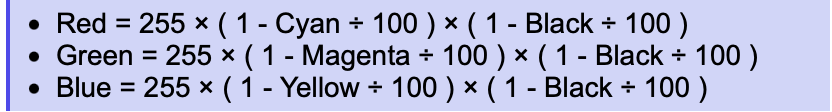
\includegraphics{images/Transfer Function values.png} 
The output graph signals are of the form 
\begin{equation*}
{\Large {s'}_{i,j}^{x'} = {a'}_{i,j}^{x'} + i*{b'}_{i,j}^{x'}} } \  where \  x' = R,G,B. 
\end{equation*}
\subsection{Image Compression using variation between pixels in neighborhood}
Now we look at compression from a different perspective, Out of the millions of pixels present in an image we start by considering many small neighbourhoods, where we compare the values of the graph signal a node with its neighbouring nodes and calculate the local variation and find out the the values which values repeat many times using the frequency analysis.\\
\newline
We can do this by using a high pass-filter to cut off the places where there is maximum repetition of a single value. We can also set a threshold {\Large $ \epsilon $ } where the image quality is compromised considering the fact that our major motive of image compression is to reduce the size of the file rather than preserving the quality of it. Now we give this value as the value for all of them because the value of {\Large $ '\epsilon' $ } is small such that the quality of image is not hindered.\\
\newline

Considering RGB colour space we get three Graph signals, One each for Red,Green and Blue now we take neighbourhood of {\Large $ '\epsilon' $ } pixels in each of the 3 components and calculate our output matrix whose cells are shifted to normalised values in each neighbourhood as mentioned above. Before if we had to store values for 'n' pixels now we only have to store it for {\Large $ n^{2}/\epsilon^{2} $ } number of pixels which is a very large number in storing hundreds and thousands of files.\\
\newline

In this method we also have a flexibility of choosing {\Large $ '\epsilon' $} to our need depending on our preference of image quality (or) file size.

The three graph signals are now subjected to Graph Fourier Transform and we now observe the outputs of each Red, Green and Blue graph signals individually. \\
\newline
an example of the three graph signal outputs is shown below: \\
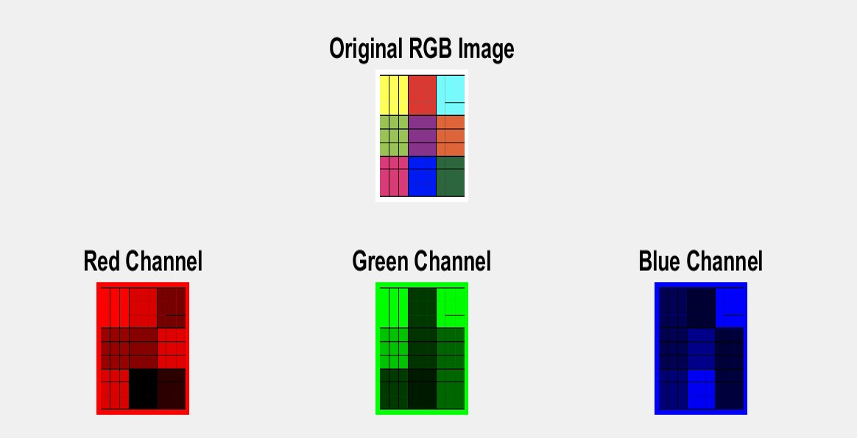
\includegraphics{images/RGB1.png} 
source: \url{ https://www.ginifab.com/feeds/pms/cmyk_to_rgb.php}
\newline

We do our neighbourhood analysis on these outputs by considering a small neighbourhood ${\Large \epislon }$ around the pixel and matching all the values to a common colour which are in the specific threshold preset by us.\\

This basically implies that small variations in the same colour are neglected and the whole neighbourhood is now considered as a single pixel in the view of efficiency of storage. As mentioned above now the no of pixels is reduced by a factor of ${\large \epsilon^{2}
}$ So our new shifted graph signals are now obtained in each neighbourhood. Where the Inverse graph Fourier Transform and inverse mapping to R,G,B values from the {\Large{s}} graph signal together give the new R,G,B values for the reduced image. \\
\newline
The frequency graph which is to be filtered is something as shown below: \\
\newline
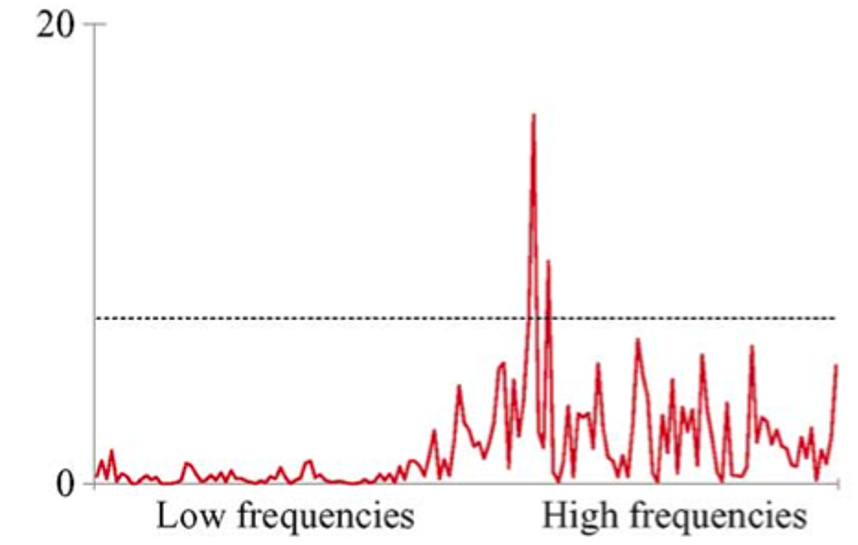
\includegraphics{images/FREQUENCY.png}  \\
\newline
Here the high frequency components are the over repeated values which are closely spaced on the real line and now we normalise these values to a single value for compression.

\section{Problem Statement}
Let us assume we have a periodic time series sinusoidal  signal of length N,then we have to find out the Graph Fourier Transform of this sinusoidal signal.
\\ \\
\newline
\textbf{SOL:} We are given a sinusoidal which is periodic so we can represent it in the form of Graph Signals as 
\begin{equation*}
    v_{0}\to v_{1}\to v_{2}\to v_{3}\to \cdots \to v_{N-1}\to v_{0} 
\end{equation*}
Lets define 
\begin{equation*}
    s = sin(w_{0}t) 
\end{equation*}
Now for this cyclic signal we have the Adjacency Matrix as
\\
\begin{equation*}
\mathcal{A} = 
\begin{bmatrix}
0 & \ & \ & \ & \ & \ & 1 \\
1 & . & \ & \ & \ & \ & \ \\
. & 1 & . & \ & \ & \ & \ \\
. & \ & . & . & \ & \ & \ \\
. & \ & \ & . & . & \ & \ \\
\ & \ & \ & \ & . & \ & \ \\
\ & \ & \ & \ & \ & 1 & 0 \\
\end{bmatrix}
\end{equation*}
\newline \\
Now we apply apply the Jordan Decomposition on this Adjacency matrix
\begin{equation*}
    \mathcal{A} = \mathcal{V} \mathcal{J} \mathcal{V}^{-1} \\
\end{equation*}
where is $\mathcal{J}$ is from the Jordan Decomposition then we obtain the matrix V which is $\mathcal{F}^{-1}$, the Fourier Transform Matrix,based on this we have the Graph Fourier Transform for the signal s to be 
\begin{equation*}
    \hat{s} = \mathcal{F}s
\end{equation*}
We have done the coding part for the above problem statement in Matlab and the results are shown below in the two graphs. The upper one is the original graph signal(s) and the lower one is the graph Fourier transform of the given graph signal s , which in this case is equivalent to the standard Fourier transform  according to the problem statement.\\
As our given signal is $ sin(w_{0}t) $ we will be having the Fourier transform of this to be two impulses at \pm {\large$w_{0}$ }. where an impulse is positive and the second is negative.

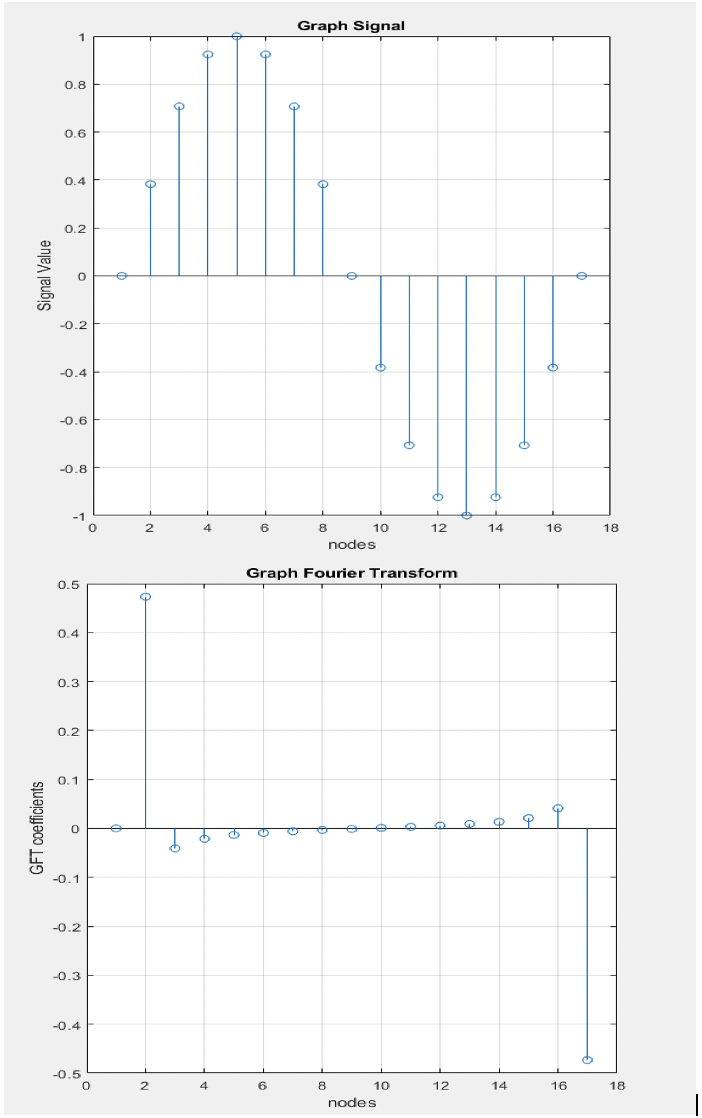
\includegraphics{images/original.png}
\newline
\section{\textbf{Conclusion}}
In this report we discussed how \textbf{Discrete time Graph Signal Processing} is done to Graph Signals. We also looked up at the Fourier Transform of Graph signals and derived expressions for them.
We discussed about the Filtering of these signals in the frequency domain.\\
We have taken up an application of Image compression using reduction in colour space and using variation between pixels in neighbourhood.Even though the results are not yet mathematically supported most of the application part is very much used in present day image compression, which educates us on how wide the applications of \textbf{Graph Signal Processing} are and how well they can be implemented.\\  

\section{\textbf{References}}
1.\url{https://ieeexplore.ieee.org/abstract/document/6808520}\\ \\
2.A. Sandryhaila and J. M. F. Moura, “Discrete signal processing on graphs: Graph Fourier transform,” in Proc. IEEE Int. Conf. Acoust., Speech, Signal Process., 2013, pp. 6167–6170 \\ \\
3.\url{https://en.wikipedia.org/wiki/Manifold#:~:text=In%20mathematics%2C%20a%20manifold%20is%20a%20topological%20space,homeomorphic%20to%20the%20Euclidean%20space%20of%20dimension%20n} \\ \\
4.\url{https://en.wikipedia.org/wiki/Riemannian_geometry}\\ \\
5.\url{https://www.ginifab.com/feeds/pms/cmyk_to_rgb.php}\\ \\
6.\url{https://in.mathworks.com/matlabcentral/answers/91036-how-do-i-split-a-color-image-into-its-3-rgb-channels}\\ \\
7.\url{https://en.wikipedia.org/wiki/RGB_color_model}\\ \\
8.\url{https://scihub.scihubtw.tw/https://www.researchgate.net/publication/317662348_The_use_of_Graph_Fourier_Transform_in_image_processing_a_new_solution_to_classical_problems?channel=doi&linkId=5947c1c3aca27242cda7e194&showFulltext=true} \\ \\
9.\url{https://www.youtube.com/watch?v=3gjJDuCAEQQ} \\ \\
10.\url{ https://arxiv.org/pdf/1712.06393.pdf} 
\end{document}


